\documentclass[%
paper=a4,%
fontsize=12pt,%
twoside=false,%
DIV18,
headsepline,
plainheadsepline,
footsepline,
plainfootsepline,
parskip=half,%
openany,%
]{scrartcl}
\usepackage[T1]{fontenc}
\usepackage[utf8]{inputenc}
\usepackage{lmodern}
\usepackage[english]{babel}
\usepackage{graphicx}
\usepackage[]{hyperref}
\title{Geany Newsletter \\[1ex]
	\small{Volume 1} \\[1ex]
	
\includegraphics{img/geany.png} \\[1.5ex]
	CC-BY}
\author{The Geany-Newsletter team}
\date{\today}
\begin{document}

\maketitle{}

\tableofcontents{}

\newpage{}

\section*{Editorial}

Welcome to the first Geany newsletter with highlights of the last few weeks
during Geany development and use. This newsletter is not intended to give a complete
overview of Geany news, but is trying to collect the most important items.
Have fun and happy coding!


\section{Geany 0.20 has been released}

On January 2011, the 6th version 0.20 of Geany "Disra" was released. As always
the release contained a number of bug fixes as well as improvements and new features.

Some of the highlights:

\begin{itemize}
	\item Improve compatibility with GVFS using GIO to save documents (Alexey Antipov).
	\item Fix occasional crashes when closing a modified document and choosing Save.
	\item Reorganise Find in Files dialog and add Files pattern to filter search results.
	\item Show mimetype icon in sidebar Documents list and notebook popup menu (Colomban Wendling).
	\item Add per-document indent width setting (Jiří Techet).
	\item Fix passing quoted arguments when using 'Send Selection to'. This means e.g. sed 's/\textbackslash{}./(dot)/g' now works.
	\item Add alternative color scheme based on Python colors (View->Editor->Color Schemes - not all filetypes supported yet).
	\item Auto-indent after an HTML/XML line without a closing tag (Eugene Arshinov).
	\item Add Forth filetype (Thomas Huth).
	\item Add Lisp filetype (Mário Silva).
	\item Add Erlang filetype (Taylor Venable).
	\item Add translations: kk.
	\item Update translations: cs, de, en\_GB, es, fi, fr, hu, ja, nl, pt, sl, sv, tr, zh\_CN.
\end{itemize}

\section{Geany-Plugins 0.20 have been released}

Shortly after the release of Geany the Geany-Plugins collection
was released with version 0.20. This collection
includes a number of useful plugins, not shipped with Geany itself.
This release is the result of about 6 months of development work
and so it has quite a number of changes and some new plugins:

\subsection{New plugins}
\subsubsection{UpdateChecker}

\textbf{UpdateChecker} implements a check for new
releases of Geany and notifies the user when one is
available. It's based on \texttt{libsoup} and can be configured to check
during startup or on request.

\subsubsection{WebHelper}

\textbf{WebHelper} is a plugin that provides some web
development facilities, such as a web page preview and some
debugging tools (web inspector). The plugin implements
the following features:

\begin{itemize}
	\item A basic web view, allowing the display of any web page (using WebKit);
	\item Possible automatic reloading of the web view upon document saving;
	\item A web inspector/debugging tool for the web view's content (including a
		JavaScript console, a viewer and editor of processed HTML and CSS, a network
		usage analysis tool and many more, thanks to WebKit).
\end{itemize}

\subsection{Updates \& Bugfixes}

Also there have been a lot of bugfixes and updates on plugins. For
further details please check the Release notes and/or the ChangeLog
of plugins. A few selected changes are:

\subsubsection{GeanyExtraSel}
\begin{itemize}
	\item Respect 'Smart' home key (Geany does now).
	\item Fixed Scintilla Shift+movement key conversion of rectangle selection.
	\item Virtual spaces support.
	\item Per-file column mode.
	\item Added "Set Anchor", "Select to Anchor" and "Rectangle Select to Anchor".
\end{itemize}

\subsubsection{GeanyGenDoc}
\begin{itemize}
	\item Bump dependency on CTPL to 0.3.
	\item Add a popup menu for common actions in the documentation type selector.
	\item Fix indentation of inserted documentation blocs.
	\item Documentation type now defaults to Doxygen (rather than nothing).
	\item Add policy PASS to completely ignore a symbol.
	\item Add basic rules for PHP.
	\item Fix build against GTK+ 2.16.
	\item Don't copy the system configuration file to the user's one when hitting
      "Edit Current Language Configuration", only write it when saving changes.
\end{itemize}

\subsubsection{GeanyLaTeX}
\begin{itemize}
	\item Move LaTeX-menu to a separate menu inside Geany main menu.
	\item Add a feature to auto-capitalize letters on typing the beginning of a sentence.
	\item Add a way to put an icon for LaTeX-wizard into Geany's main toolbar.
	\item Added a dialog for inserting BibTeX references based on available *.bib-files.
\end{itemize}

\subsubsection{TreeBrowser}
\begin{itemize}
	\item Added bookmarks support.
	\item Added keybindings support.
	\item Added mime type icons in the tree.
	\item Many bugfixes and code improvements.
\end{itemize}

\section{Geany-Development}

After the 0.20 release the development has slowed down a bit but
nevertheless, some changes did happen:

\subsection{Update to Scintilla 2.22}

Right after the release of Geany 0.20 with Subversion r5521 an
updated version of Scintilla was been merged from the unstable branch
into trunk. Geany trunk is now running with version 2.22 of
the Scintilla editing component.

\subsection{Further patches}
\subsubsection{Support for COBOL}

At the end of January 2011 a patch was committed to Geany trunk which
enabled COBOL support inside Geany. Now it's possible to use
features like syntax highlighting for this language.


\section{Plugins}

It was a quite active time right after the 0.20 release on the plugin
development side.

\subsection{New plugins to Geany-Plugins-project}
\subsubsection{Tableconvert}

After a little chaos with naming, the new plugin \textbf{Tableconvert}
was added to the development version of the Geany-Plugins. It
offers a way to convert tab separated lists (e.g. imported
from Microsoft Excel or Libreoffice Calc) into a table. Currently the
plugin supports HTML and \LaTeX{} tables.

\subsubsection{Debugger}

The \textbf{Debugger} plugin has added a second binding for gdb to
the Geany-Plugins project.

\subsubsection{GeanyPG}

With \textbf{GeanyPG} Hans Alves submitted a new plugin to
geany-plugins project which adds support for signing,
encrypting and decryption of text files opened in Geany.

\section{Geany Universe}

\subsection{New Mailing List -- geany-newsletter-commits}

When the \texttt{geany-newsletter} project was started, a
a new commit mailing was created. The goal of this list is
to notify all interested people whenever a new commit has taken place
inside the geany-newsletter git repository. As always you can find
the list via \url{http://www.geany.org/Support/MailingList}

\subsection{New team member -- Colomban Wendling}

In March 2011, Colomban Wendling joined the Geany core team. Over
the last few years he has submitted a lot of patches. He did a great
job during the last month - e.g. building up a tagmanager-in-memory
patchset as well as providing a big number of patches and providing
support on both the mailing list as well as IRC. Welcome Colomban!

\subsection{Geany local}
\subsubsection{Geany at Chemnitzer Linuxtage 2011 (March 19th, 20th)}

On the coming weekend (around March 19th, 20th) there will be a local Linux and FOSS
convention in Chemnitz, Germany. Some of the Geany guys will be
around and have a little table during this event. So if you are nearby, come
join us for a chat. You will find us next to the Xfce guys.

Details for this convention can be find on their homepage at \url
{http://chemnitzer.linux-tage.de/2011/}

\section{Let us introduce you....}

This section is intended to introduce particular plugins or
features on a regular basis.

\subsection{Plugin Focus}
\subsubsection{File Browser}

The \textbf{File Browser} plugins adds to the sidebar a tab with
which you can browser files and folders. By default it shows the
contents of the folder containing the first file opened in Geany.
You can navigate to other drives and folders using any of the
options available at the very top of the tab:

\textbf{Up:} Navigates to one folder higher in the file system.

\textbf{Home:} Navigates to your Home folder.

\textbf{Set path from document:} Sets the active folder to the one
containing the current active document.

\textbf{Folder input box:} Here you can enter any path you want to
see in the File Browser. As you type the path it will offer
autocompletion of the folder's name.

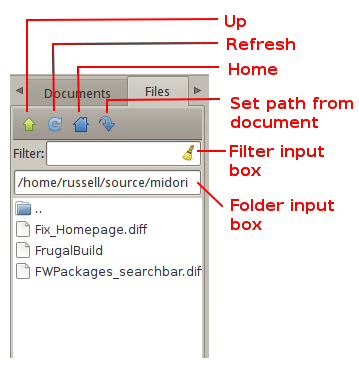
\includegraphics[width=5cm]{img/issue1_filebrowser.png}

Also at the top of the tab is the Filter input box in which you can
enter a file specification of those files you want to appear in the
File Browser. The file specifications must be quite simple - e.g.
g*.py or *.xml. Regular expressions are not supported. To clear the
filter either click on the icon at the right of the Filter input box
or empty the Filter box and press [Enter].



\subsection{Feature Focus}

\subsubsection{Comments formatting}

When writing source code or in a markup language, it's often
necessary to mark one or more lines as a comment. Geany offers
several functions from the Edit > Format sub-menu which make this
very easy:

\begin{itemize}
	\item Comment Line(s)
	\item Uncomment Line(s)
	\item Toggle Line Commentation
\end{itemize}

To use these options on a single line, put the cursor on that line
and select the menu option. To use them on a block of code, select
the whole block then select the menu option. The Toggle Line
Commentation menu option will, as its name suggests, add comment
markers to a normal line/section of code and, if the line/section is
already a comment, remove the comment markers. What's great about
these options is that they insert or remove the comment markers
applicable to the type of file being edited. This means that you can
focus on the content of what you're editing instead of having to
worry about getting the comment markers right. This is precisely
Geany's aim: to make coding easier and faster without getting in
your way.

\section{Contact}

If you like to contribute to the newsletter, make a request or
complaint about content please contact frank@geany.org via email.

\end{document}
